\label{sec:pileup}

The pileup dependence of the jet mass for the various grooming
algorithms is now investigated. Figure~\ref{figs:histAK7MjetVsNvtx_nvtxPlots} shows
the average jet mass as a function of the number of primary vertices,
for all of the various grooming techniques, compared to the ungroomed
jets. Data are shown as solid lines and the Monte Carlo are shown
as hatched lines. The same grooming techniques have the same
colors. The ungroomed jets are shown in black. The filtered jets are
shown in red. The trimmed jets are shown in blue. The pruned jets
are shown in green. Since the $\pt$ spectrum of the jets in the
MC is different from that of the data in the dijet sample, there
is a disagreement between the central values of the distribution. 


\begin{figure}[htbp]
\centering
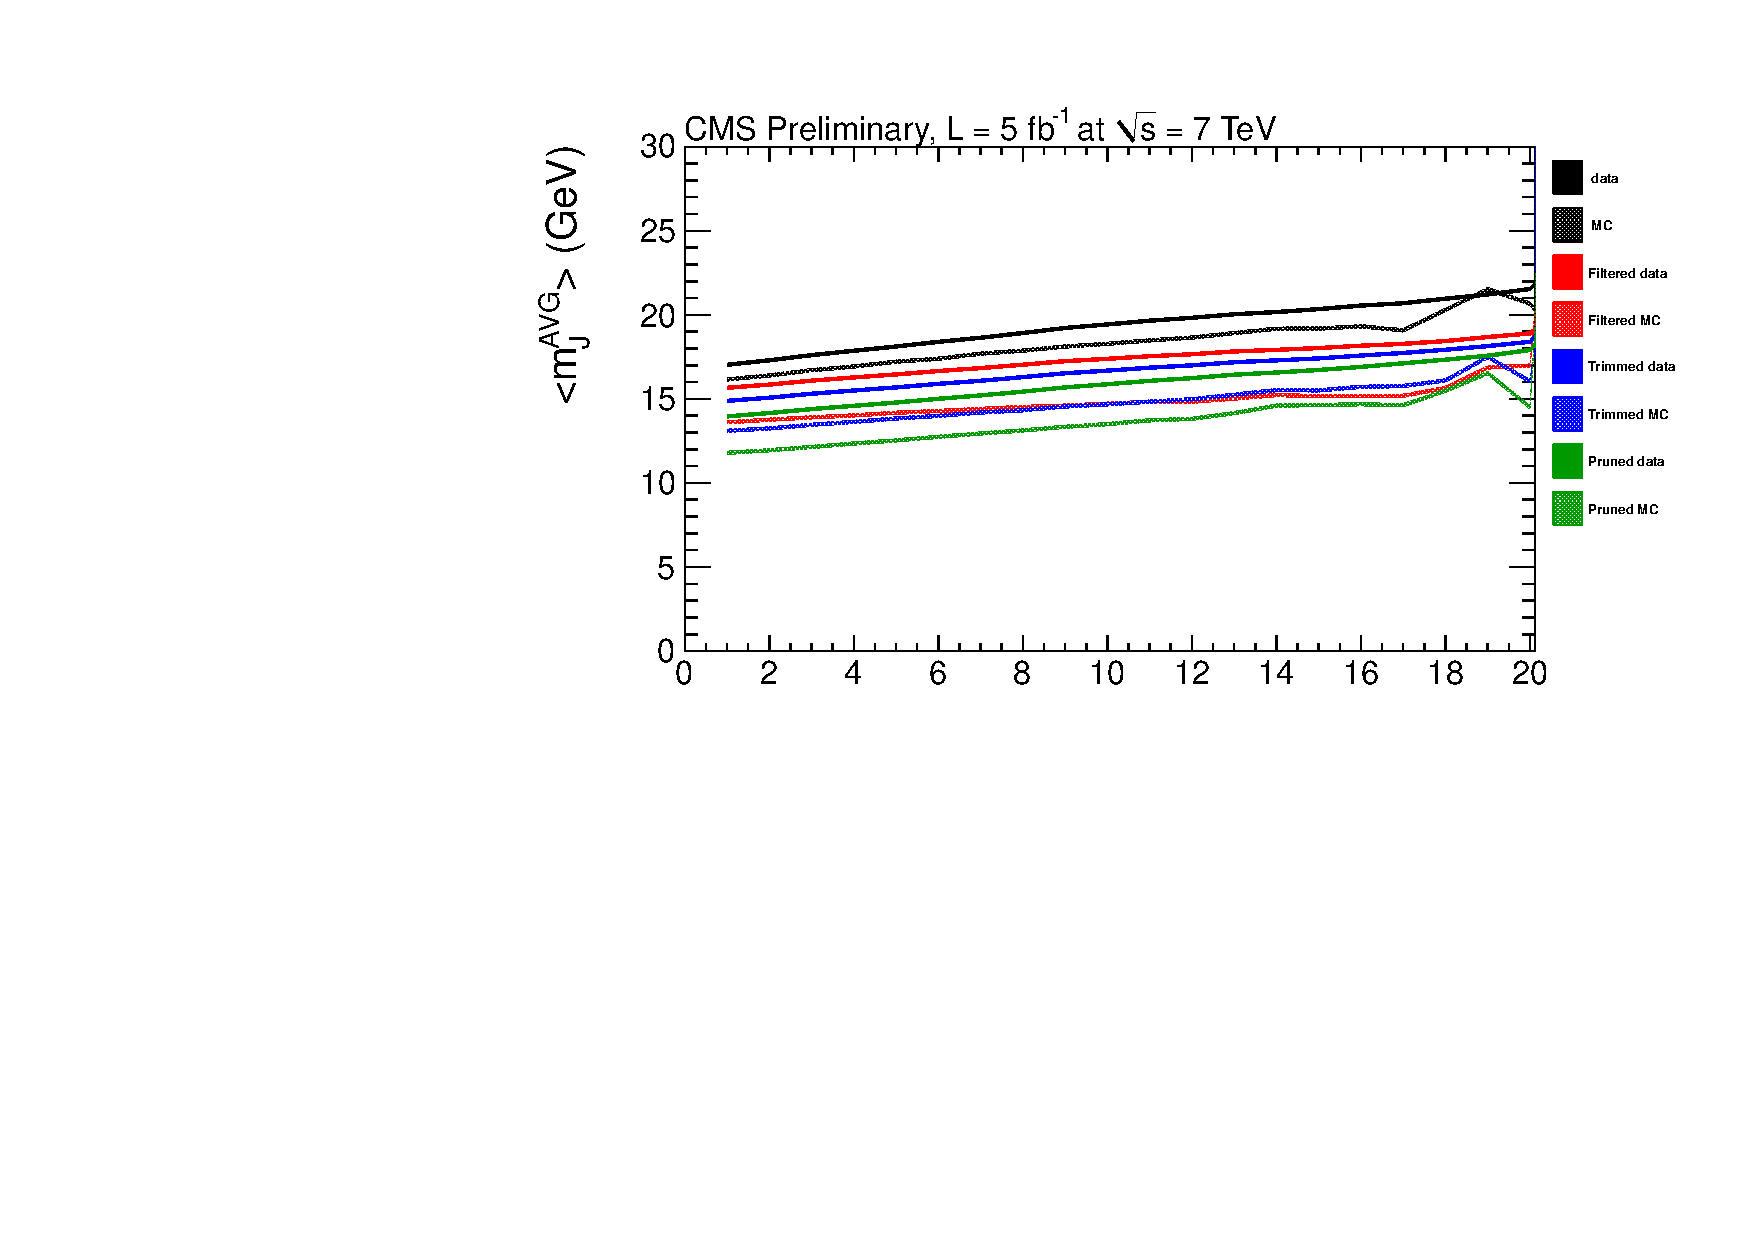
\includegraphics[width=0.95\textwidth]{figs/histAK7MjetVsNvtx_nvtxPlots}
\caption{Detector-level distributions of the average jet mass for AK7 jets,
for all grooming algorithms as well as the ungroomed distribution,
as a function of the number of reconstructed primary vertices. 
\label{figs:histAK7MjetVsNvtx_nvtxPlots}}
\end{figure}

